% Presentacion autocontenida. Compilar dos veces con pdfLaTeX.
\documentclass[aspectratio=169,11pt]{beamer}
\usepackage[utf8]{inputenc}
\usepackage[T1]{fontenc}
\usepackage[provide=*,spanish]{babel}
\usepackage{lmodern,amsmath,amssymb,booktabs,tabularx,tikz,pgfplots}
\pgfplotsset{compat=1.18}
\definecolor{navy}{HTML}{16324F}
\definecolor{teal}{HTML}{007F82}
\definecolor{pale}{HTML}{EDF5F5}
\definecolor{graytext}{HTML}{526273}
\setbeamercolor{normal text}{fg=navy,bg=white}
\setbeamercolor{structure}{fg=teal}
\setbeamercolor{frametitle}{fg=navy}
\setbeamercolor{title}{fg=navy}
\setbeamercolor{block title}{fg=white,bg=teal}
\setbeamercolor{block body}{fg=navy,bg=pale}
\setbeamerfont{frametitle}{size=\Large,series=\bfseries}
\setbeamertemplate{frametitle}{\vspace{0.25cm}\raggedright\insertframetitle\par\vspace{0.15cm}}
\setbeamertemplate{navigation symbols}{}
\setbeamertemplate{itemize items}[circle]
\setbeamertemplate{footline}{\hfill\textcolor{graytext}{\scriptsize RK4 vectorial\quad\insertframenumber/\inserttotalframenumber}\hspace{0.6cm}\vspace{0.25cm}}
\setbeamersize{text margin left=0.8cm,text margin right=0.8cm}
\newcommand{\R}{\mathbb R}\newcommand{\E}{\mathbb E}
\newcommand{\norm}[1]{\left\lVert#1\right\rVert}
\newcommand{\source}[1]{\vfill{\tiny\color{graytext}#1}}
\title{RK4 para sistemas vectoriales}
\subtitle{Condiciones iniciales aleatorias y paso adaptativo}
\author{José Carlos Torres Donaire}
\institute{Universidad Nacional Autónoma de Honduras}
\date{13 de octubre de 2026}
\begin{document}
\begin{frame}[plain]
\vspace{0.6cm}
{\color{teal}\small ANÁLISIS NUMÉRICO}\par\vspace{0.5cm}
{\color{navy}\fontsize{28}{32}\selectfont\bfseries RK4 para sistemas\par vectoriales}\par\vspace{0.5cm}
{\Large Condiciones iniciales aleatorias\par y paso adaptativo}\par\vspace{0.7cm}
\textcolor{teal}{\rule{12.7cm}{1pt}}\par\vspace{0.3cm}
José Carlos Torres Donaire\par
{\small Universidad Nacional Autónoma de Honduras\par13 de octubre de 2026}
\end{frame}

\begin{frame}{Problema y objetivos}
\[
u'(t,\omega)=f(t,u(t,\omega)),\quad u(t_0,\omega)=U_0(\omega),
\qquad f:I\times\R^d\to\R^d.
\]
\begin{itemize}
\item Desarrollar RK4 para dimensión arbitraria y componentes acopladas.
\item Propagar una ley inicial sin imponer gaussianidad ni linealidad.
\item Derivar un controlador de paso a partir del error local.
\item Conectar el análisis con literatura primaria y experimentos reproducibles.
\end{itemize}
\begin{block}{Alcance}
La teoría se formula para una clase general. Los ejemplos verifican el método
bajo hipótesis declaradas y no restringen su definición.
\end{block}
\end{frame}

\begin{frame}{La fuente de aleatoriedad determina el algoritmo}
\renewcommand{\arraystretch}{1.35}
\begin{tabularx}{0.98\linewidth}{@{}p{3.2cm}XX@{}}\toprule
Fuente & Qué varía & Tratamiento\\\midrule
Dato inicial & $U_0$ según una ley prescrita & RK4 por realización\\
Error numérico & Aproximación del flujo & Refinamiento y estimación del error\\
Ruido dinámico & Incrementos de $W(t)$ & Método para una EDS, como Euler--Maruyama\\\bottomrule
\end{tabularx}\par
\vspace{0.4cm}
\[
u(t,\omega)=\varphi_{t,t_0}(U_0(\omega)),\qquad
\mu_t=(\varphi_{t,t_0})_\#\mu_0.
\]
Una entrada aleatoria produce una familia de EDO deterministas condicionadas
al dato inicial.
\end{frame}

\begin{frame}{Hipótesis que permiten cuarto orden}
\begin{itemize}
\item Continuidad y Lipschitz local en el estado para existencia y unicidad local.
\item Ausencia de explosión antes del tiempo final.
\item Regularidad $C^5$ y derivadas acotadas en la región de trayectorias y etapas.
\item Control Lipschitz de la aplicación numérica y de los defectos locales.
\end{itemize}
\[
\norm{\varphi_{t,t_0}(z)-\varphi_{t,t_0}(w)}
\leq e^{L(t-t_0)}\norm{z-w}.
\]
\begin{block}{Sensibilidad}
La dinámica puede amplificar tanto la incertidumbre inicial como los errores
de integración. El horizonte temporal forma parte de la garantía.
\end{block}
\source{Marco clásico: Hairer, Nørsett y Wanner, Solving ODEs I, 2.ª ed., 1993.}
\end{frame}

\begin{frame}{RK4 usa cuatro vectores de etapa}
\begin{align*}
k_1&=h f(t,u),&
k_2&=h f(t+h/2,u+k_1/2),\\
k_3&=h f(t+h/2,u+k_2/2),&
k_4&=h f(t+h,u+k_3).
\end{align*}
\[
u_{\mathrm{nuevo}}=u+\frac{k_1+2k_2+2k_3+k_4}{6}.
\]
\begin{columns}[T]
\begin{column}{0.46\textwidth}
\[
\begin{array}{c|rrrr}
0&0&0&0&0\\
1/2&1/2&0&0&0\\
1/2&0&1/2&0&0\\
1&0&0&1&0\\\hline
&1/6&1/3&1/3&1/6
\end{array}
\]
\end{column}
\begin{column}{0.49\textwidth}
\vspace{0.3cm}
Cada $k_i$ incluye $h$.\par\vspace{0.2cm}
Todas las componentes usan el mismo vector de etapa.\par\vspace{0.2cm}
El sistema puede ser no lineal y no autónomo.
\end{column}
\end{columns}
\end{frame}

\begin{frame}{Las ocho condiciones de orden se verifican exactamente}
\small
\begin{columns}[T]
\begin{column}{0.47\textwidth}
\begin{align*}
b^\top\mathbf1&=1,\\
b^\top c&=1/2,\\
b^\top c^2&=1/3,\\
b^\top Ac&=1/6.
\end{align*}
\end{column}
\begin{column}{0.47\textwidth}
\begin{align*}
b^\top c^3&=1/4,\\
b^\top CAc&=1/8,\\
b^\top Ac^2&=1/12,\\
b^\top A^2c&=1/24.
\end{align*}
\end{column}
\end{columns}
\vspace{0.4cm}
$c=A\mathbf1$, $C=\operatorname{diag}(c)$ y las potencias son componente a componente.
\begin{block}{Conclusión algebraica}
Las expansiones del flujo y del método coinciden hasta grado cuatro para
sistemas vectoriales. El defecto local es $O(h^5)$ bajo las hipótesis de suavidad.
\end{block}
\end{frame}

\begin{frame}{La convergencia también vale en mallas no uniformes}
Sea $h_* =\max_n h_n$, $\sum_n h_n=T-t_0$ y $K\geq0$. Para el error $e_n$,
\[
e_{n+1}\leq (1+Kh_n)e_n+C_{\mathrm{loc}}h_n^5.
\]
La recurrencia y Grönwall discreto implican
\[
\boxed{\max_n e_n\leq e^{K(T-t_0)}
\bigl(e_0+C_{\mathrm{loc}}(T-t_0)h_*^4\bigr).}
\]
\begin{itemize}
\item La suma de defectos usa $\sum_n h_n^5\leq h_*^4(T-t_0)$.
\item Con $e_0=0$, el orden global es cuatro.
\item Las constantes deben controlar toda la región de etapas.
\end{itemize}
\end{frame}

\begin{frame}{RK4 conserva una restricción de estabilidad explícita}
\[
R_{\mathrm{RK4}}(z)=1+z+z^2/2+z^3/6+z^4/24,
\quad z=h\lambda.
\]
\renewcommand{\arraystretch}{1.3}
\small
\begin{tabularx}{0.98\linewidth}{@{}lXX@{}}\toprule
Método & Orden global & Intervalo real de estabilidad\\\midrule
Euler explícito & 1 & $[-2,0]$\\
RK4 clásico & 4 & $[-2.785293,0]$ aproximadamente\\\bottomrule
\end{tabularx}\par
\par\vspace{0.45cm}
Para $u'=Au$, la matriz de propagación es $R(hA)$.
\begin{itemize}
\item La no normalidad puede producir crecimiento transitorio.
\item La rigidez puede imponer pasos pequeños incluso con tolerancia holgada.
\item Adaptar $h$ no convierte RK4 en un método A-estable.
\end{itemize}
\end{frame}

\begin{frame}{La ley inicial se transporta por el flujo}
\[
U_0\sim\mu_0,\qquad u(t)=\varphi_{t,t_0}(U_0),\qquad
\mu_t=(\varphi_{t,t_0})_\#\mu_0.
\]
\begin{itemize}
\item Muestrear $U_0$ una vez por trayectoria.
\item Mantener ese dato durante todas las etapas y todos los pasos.
\item Comparar trayectorias en tiempos físicos comunes.
\end{itemize}
\[
m'(t)=\E[f(t,u(t))].
\]
En un sistema no lineal esta esperanza no se obtiene, en general, evaluando
$f$ en la media. La evolución de momentos puede requerir momentos superiores.
\end{frame}

\begin{frame}{La garantía probabilística requiere integrabilidad}
Si, casi seguramente,
\[
\max_n\norm{u(t_n,\omega)-U_n(\omega)}
\leq C(\omega)h_*(\omega)^4,
\]
y $C\in L^p$, $h_*(\omega)\leq\varepsilon$, entonces
\[
\left\|\max_n\norm{u(t_n)-U_n}\right\|_{L^p}
\leq\norm{C}_{L^p}\varepsilon^4.
\]
En un tiempo final común, el mismo acoplamiento da
\[
W_p(\mathcal L(u(T)),\mathcal L(U_T))\leq\norm{C}_{L^p}\varepsilon^4.
\]
\small Soporte compacto facilita cotas uniformes. Para una ley gaussiana hay
que controlar crecimiento y momentos, o truncar con una cota de colas.
\end{frame}

\begin{frame}{Monte Carlo agrega un error diferente al temporal}
Para una cantidad de interés $q$ y realizaciones independientes,
\[
Q_M^h=\frac1M\sum_{j=1}^M q(U_T^{(j)}),\qquad
Q=\E[q(u(T))].
\]
\[
\E[(Q_M^h-Q)^2]
=\frac{\operatorname{Var}(q(U_T))}{M}
+\bigl(\E[q(U_T)]-Q\bigr)^2.
\]
\begin{block}{Balance de errores}
Para $q$ Lipschitz, varianza uniformemente finita y RK4 bajo sus hipótesis, el error RMS es
$O(M^{-1/2}+h_*^4)$. Reducir el paso aporta poco si el muestreo domina.
\end{block}
\small Un intervalo estadístico convencional no incorpora automáticamente
sesgo temporal ni error de modelo.
\end{frame}

\begin{frame}{Duplicar el paso produce el factor 15}
\[
y_c=\Psi_h(t,y),\quad
y_f=\Psi_{h/2}(t+h/2,\Psi_{h/2}(t,y)).
\]
En el régimen asintótico,
\[
y_c=y_*+Ch^5+O(h^6),\qquad
y_f=y_*+\frac{C}{16}h^5+O(h^6).
\]
\[
\boxed{\widehat e_f=(y_f-y_c)/15=y_*-y_f+O(h^6).}
\]
Se acepta $y_f$, conservando orden global cuatro. Agregar la corrección
de Richardson constituye una variante distinta del método.
\end{frame}

\begin{frame}{La norma escalada gobierna aceptación y rechazo}
\[
s_i=\mathrm{atol}_i+\mathrm{rtol}\max(|y_i|,|(y_f)_i|),\qquad
r=\max_i\frac{|(\widehat e_f)_i|}{s_i}.
\]
\begin{columns}[T]
\begin{column}{0.47\textwidth}
\begin{block}{$r\leq1$}
Aceptar $y_f$ y avanzar el tiempo.
\end{block}
\end{column}
\begin{column}{0.47\textwidth}
\begin{block}{$r>1$}
Conservar $(t,y)$ y repetir con menor paso.
\end{block}
\end{column}
\end{columns}
\vspace{0.3cm}
\[
h_{\mathrm{nuevo}}=h\,\operatorname{clip}(0.9r^{-1/5},0.2,5).
\]
\small El exponente $1/5$ viene del estimador local. La tolerancia regula ese
estimador y no certifica una cota absoluta global.
\end{frame}

\begin{frame}{El controlador y el estimador forman parte del método}
\begin{itemize}
\item RK4 clásico tiene cuatro etapas y carece de estimador embebido por definición.
\item Duplicación directa cuesta doce evaluaciones por intento.
\item Dormand--Prince 5(4) comparte etapas para una pareja de órdenes cinco y cuatro.
\item PI/PID incorporan historial y pueden mejorar estabilidad del control del paso.
\end{itemize}
\[
h_{n+1}=h_n\gamma r_n^{-\alpha/5}r_{n-1}^{\beta/5}
\quad\text{con limitadores y parámetros justificados.}
\]
\source{Dormand y Prince (1980), DOI 10.1016/0771-050X(80)90013-3.
Ranocha y Giesselmann (2024), arXiv:2307.12677.}
\end{frame}

\begin{frame}{La malla del ensamble exige tiempos de observación comunes}
La realización $j$ puede aceptar una secuencia distinta $t_n^{(j)}$.
\begin{itemize}
\item El mismo índice de nodo no implica el mismo tiempo físico.
\item Forzar llegada a tiempos de observación evita mezclar estados asincrónicos.
\item Una salida densa debe mantener orden compatible con el integrador.
\item Interpolación lineal puede reducir la precisión a segundo orden.
\end{itemize}
\begin{block}{Error probabilístico}
Las mallas dependientes de $U_0$ se analizan trayectoria por trayectoria,
con control del máximo paso y de las constantes aleatorias.
\end{block}
\end{frame}

\begin{frame}{Euler--Maruyama corresponde a ruido en la dinámica}
\[
\mathrm dX=a(t,X)\,\mathrm dt+B(t,X)\,\mathrm dW,
\qquad B\in\R^{d\times m}.
\]
\[
X_{n+1}=X_n+h\,a(t_n,X_n)+B(t_n,X_n)\Delta W_n,
\quad\Delta W_n\sim\mathcal N(0,hI_m).
\]
\begin{itemize}
\item Orden fuerte genérico $1/2$ con Lipschitz, crecimiento y regularidad apropiada.
\item Orden débil uno bajo hipótesis adicionales de suavidad y momentos.
\item Con difusión nula recupera Euler determinista.
\item Añadir ruido a RK4 no conserva automáticamente cuarto orden estocástico.
\end{itemize}
\source{Higham (2001), SIAM Review 43(3), 525--546, DOI 10.1137/S0036144500378302.}
\end{frame}

\begin{frame}{El refinamiento estocástico debe conservar el camino}
Si se observa $\Delta W$ y luego se divide un paso,
\[
\Delta W_1=\tfrac12\Delta W+\sqrt{h/4}\,Z,
\qquad \Delta W_2=\Delta W-\Delta W_1,
\quad Z\sim\mathcal N(0,I_m).
\]
$Z$ es independiente del incremento original y de la información pasada.
\begin{itemize}
\item El puente browniano conserva la suma del incremento original.
\item Descartar ruido tras un rechazo dependiente del ruido puede introducir sesgo.
\item El código entregado usa malla determinista para Euler--Maruyama.
\end{itemize}
\begin{block}{Distinción operativa}
El rechazo adaptativo determinista de RK4 necesita una justificación nueva
antes de trasladarse a una EDS.
\end{block}
\end{frame}

\begin{frame}{Estado del arte: incertidumbre y aleatorización}
\small\renewcommand{\arraystretch}{1.35}
\begin{tabularx}{0.98\linewidth}{@{}p{3.5cm}X@{}}\toprule
Trabajo & Conexión con la asignación\\\midrule
Schober et al., 2014 & Medias probabilísticas ligadas a métodos RK; incertidumbre numérica.\\
Conrad et al., 2015 & Medidas sobre soluciones numéricas mediante aleatorización.\\
Kruse y Wu, 2017 & RK aleatorizados para irregularidad temporal, distinto de dato inicial aleatorio.\\
Abdulle y Garegnani, 2020 & Pasos aleatorios para incertidumbre de discretización y estructura geométrica.\\\bottomrule
\end{tabularx}\par
\par\vspace{0.3cm}
\small Estas líneas no se identifican automáticamente con RK4 aplicado a $U_0$.
\source{arXiv:1406.2582, 1506.04592, 1701.03444 y 1801.01340.}
\end{frame}

\begin{frame}{Estado del arte: control, calibración y estructura}
\small\renewcommand{\arraystretch}{1.35}
\begin{tabularx}{0.98\linewidth}{@{}p{3.7cm}X@{}}\toprule
Trabajo & Contribución pertinente\\\midrule
Bosch et al., 2021 & Calibración de filtros probabilísticos con selección adaptativa de paso.\\
Ranocha y Giesselmann, 2024 & Estimadores por residuos y estabilidad de controladores I, PI y PID.\\
Bleecke y Ranocha, 2023 & Relajación para preservar invariantes junto con adaptatividad.\\
Wu y Lysy, 2025 & \emph{rodeo}: integración probabilística e inferencia paramétrica.\\\bottomrule
\end{tabularx}\par
\vspace{0.3cm}
\small Las garantías y los costos dependen de las hipótesis de cada enfoque.
\source{arXiv:2012.08202, 2307.12677, 2311.14050 y 2506.21776.}
\end{frame}

\begin{frame}{Trazabilidad y alcance bibliográfico}
\begin{itemize}
\item Revisión narrativa selectiva, consultada el 13 de octubre de 2026.
\item Selección central 2014--2025, con antecedentes clásicos.
\item Metadatos y resúmenes primarios contrastados. Consulta de textos HTML sobre control por residuos, calibración y \emph{rodeo}.
\item Connected Papers permitió localizar pistas públicas, pero no se obtuvo una exportación verificable de su grafo interactivo.
\end{itemize}
\begin{block}{Semillas pertinentes para reproducir la exploración}
\texttt{2012.08202}: calibración e incertidumbre.\par
\texttt{2307.12677}: estimación y control adaptativo.
\end{block}
\small La matriz de conexiones es una síntesis temática propia, no una
representación de aristas verificadas de Connected Papers.
\end{frame}

\begin{frame}{Un sistema acoplado de ocho variables confirma cuarto orden}
\begin{columns}
\begin{column}{0.57\textwidth}
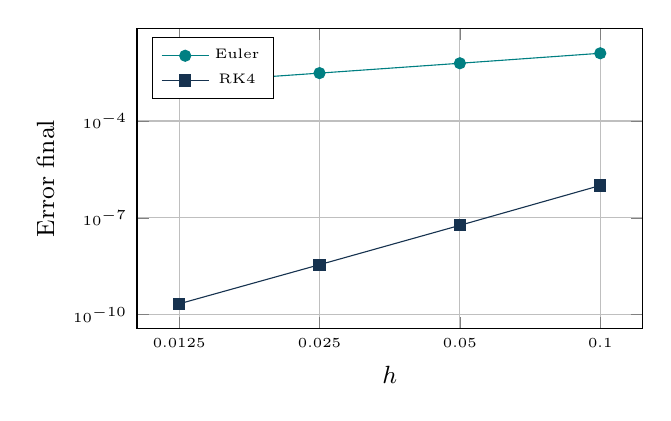
\begin{tikzpicture}
\begin{loglogaxis}[width=8cm,height=5.4cm,xtick={0.0125,0.025,0.05,0.1},xticklabels={0.0125,0.025,0.05,0.1},minor x tick num=0,xlabel={$h$},ylabel={Error final},grid=both,legend pos=north west,legend style={font=\tiny},tick label style={font=\tiny},label style={font=\small}]
\addplot[teal,mark=*] coordinates{(0.1,0.01248969)(0.05,0.00613136)(0.025,0.00303751)(0.0125,0.00151174)};\addlegendentry{Euler}
\addplot[navy,mark=square*] coordinates{(0.1,1.0068177e-6)(0.05,5.876886e-8)(0.025,3.549841e-9)(0.0125,2.181144e-10)};\addlegendentry{RK4}
\end{loglogaxis}\end{tikzpicture}
\end{column}
\begin{column}{0.39\textwidth}
\small
$u'=Au+B\tanh(u)+0.2\sin(\nu t)$\par\vspace{0.3cm}
Órdenes observados finales:\par
\textbf{Euler: 1.007}\par
\textbf{RK4: 4.025}\par\vspace{0.3cm}
Referencia independiente DOP853. Diferencia entre dos refinamientos:
$2.19\times10^{-15}$.
\end{column}
\end{columns}
\source{Cálculos ejecutados para este trabajo. Semilla 20261013.}
\end{frame}

\begin{frame}{La adaptación reduce el error con mayor costo}
\small\renewcommand{\arraystretch}{1.3}
\begin{tabularx}{0.98\linewidth}{@{}lrrrr@{}}\toprule
$\mathrm{rtol}$ & Aceptados & Rechazos & Eval. $f$ & Error máximo\\\midrule
$10^{-3}$ & 20 & 0 & 240 & $4.727\cdot10^{-5}$\\
$10^{-5}$ & 28 & 6 & 408 & $3.631\cdot10^{-6}$\\
$10^{-7}$ & 56 & 15 & 852 & $1.121\cdot10^{-7}$\\
$10^{-9}$ & 138 & 22 & 1920 & $2.787\cdot10^{-9}$\\\bottomrule
\end{tabularx}\par
\vspace{0.35cm}
Familia verificable para cualquier dato inicial:
\[
u'=A(u-g)+g',\qquad u(t)=g(t)+e^{At}(u_0-g(0)).
\]
\small $g$ contiene un pulso suave. Error medido en nodos aceptados.
$h_{\max}=0.1$ y $\mathrm{atol}=10^{-3}\mathrm{rtol}$.
\source{Resultados propios, sin extrapolación de Richardson.}
\end{frame}

\begin{frame}{En el ensamble domina el error de muestreo}
\[
U_0\sim\mathcal N(\mu,\Sigma_0),\qquad u'=Au,\qquad
M=20\,000,\quad h=0.05.
\]
\renewcommand{\arraystretch}{1.4}
\small
\begin{tabularx}{0.98\linewidth}{@{}Xr@{}}\toprule
Medición emparejada & Valor\\\midrule
Error numérico de la media & $2.699\cdot10^{-8}$\\
Error de muestreo de la media & $7.284\cdot10^{-4}$\\
RMS del error de trayectoria & $3.292\cdot10^{-8}$\\\bottomrule
\end{tabularx}\par
\par\vspace{0.4cm}
La solución exacta y RK4 usan las mismas realizaciones iniciales.
Este acoplamiento separa el efecto temporal del estadístico.
\par\vspace{0.2cm}
\small La auditoría combinó dato aleatorio y paso adaptativo en 32 trayectorias
no lineales de ocho variables. Máximo error final: $7.638\cdot10^{-8}$.
\source{El sistema lineal sirve como verificación con momentos exactos. El algoritmo es general.}
\end{frame}

\begin{frame}{Euler--Maruyama muestra orden fuerte cercano a un medio}
\small\renewcommand{\arraystretch}{1.25}
\begin{tabular}{@{}rrrr@{}}\toprule
Pasos & RMSE fuerte & Orden & Sesgo débil exacto\\\midrule
32 & $5.879\cdot10^{-2}$ & --- & $1.048\cdot10^{-3}$\\
64 & $4.022\cdot10^{-2}$ & 0.548 & $5.223\cdot10^{-4}$\\
128 & $2.880\cdot10^{-2}$ & 0.482 & $2.608\cdot10^{-4}$\\
256 & $2.068\cdot10^{-2}$ & 0.478 & $1.303\cdot10^{-4}$\\
512 & $1.467\cdot10^{-2}$ & 0.496 & $6.513\cdot10^{-5}$\\
1024 & $1.027\cdot10^{-2}$ & 0.514 & $3.256\cdot10^{-5}$\\\bottomrule
\end{tabular}\par
\vspace{0.3cm}
\small Test: $\mathrm dX=-0.3X\,\mathrm dt+0.7X\,\mathrm dW$, $X_0=1$.
12\,000 caminos con incrementos finos sumados para todas las mallas.
El sesgo débil de la media se calcula analíticamente.
\end{frame}

\begin{frame}{Conclusiones}
\begin{itemize}
\item RK4 alcanza cuarto orden vectorial bajo regularidad y control de estabilidad.
\item El dato inicial aleatorio se propaga por el flujo y requiere cotas integrables para garantías $L^p$.
\item La duplicación proporciona el factor 15 y el controlador con exponente $1/5$.
\item La tolerancia local, el error global y el error Monte Carlo deben medirse por separado.
\item Euler--Maruyama incorpora ruido dinámico y exige un análisis estocástico distinto.
\end{itemize}
\begin{block}{Siguiente paso metodológico}
Comparar costo frente a error con pares embebidos y controladores PI,
manteniendo trazabilidad de hipótesis, rechazos y cantidades de interés.
\end{block}
\end{frame}

\begin{frame}{Referencias para ampliar el análisis}
\footnotesize
\begin{itemize}
\item Hairer, Nørsett y Wanner (1993). \emph{Solving ODEs I}.
DOI: \href{https://doi.org/10.1007/978-3-540-78862-1}{10.1007/978-3-540-78862-1}.
\item Dormand y Prince (1980). Pares RK embebidos.
DOI: \href{https://doi.org/10.1016/0771-050X(80)90013-3}{10.1016/0771-050X(80)90013-3}.
\item Higham (2001). Integración estocástica.
DOI: \href{https://doi.org/10.1137/S0036144500378302}{10.1137/S0036144500378302}.
\item Schober et al. (2014): \href{https://arxiv.org/abs/1406.2582}{arXiv:1406.2582}.
Conrad et al. (2015): \href{https://arxiv.org/abs/1506.04592}{arXiv:1506.04592}.
\item Kruse y Wu (2017): \href{https://arxiv.org/abs/1701.03444}{arXiv:1701.03444}.
Abdulle y Garegnani (2020): \href{https://arxiv.org/abs/1801.01340}{arXiv:1801.01340}.
\item Bosch et al. (2021): \href{https://arxiv.org/abs/2012.08202}{arXiv:2012.08202}.
Ranocha y Giesselmann (2024): \href{https://arxiv.org/abs/2307.12677}{arXiv:2307.12677}.
\item Bleecke y Ranocha (2023): \href{https://arxiv.org/abs/2311.14050}{arXiv:2311.14050}.
Wu y Lysy (2025): \href{https://arxiv.org/abs/2506.21776}{arXiv:2506.21776}.
\end{itemize}
\small Bibliografía completa y alcance de lectura en el informe técnico.
\end{frame}
\end{document}
